\subsection{Water suppression}
\label{subsec:poise__solvsupp}

The suppression of solvent signals is one of the most important techniques in modern NMR, especially in cases where solvent deuteration is not a viable strategy (e.g.\ when exchangeable protons must be observed).\autocite{Zheng2010PNMRS,Giraudeau2015M}
Here, we specifically seek to optimise the 1D NOESY experiment with presaturation\autocite{Mckay2011CMR} (\cref{fig:poise_solvsupp_pulseq}): although this sequence is popular, its performance can depend on at least four parameters, namely the transmitter offset, presaturation power, the NOE mixing time, and the presaturation duration or recovery delay.
In this section, I use the symbols $\nu_\text{tx}$, $k$, $\taum$, and $\taur$ to respectively refer to these four parameters: the corresponding TopSpin parameters are \texttt{O1}, \texttt{CNST20}, \texttt{D8}, and \texttt{D1}.

\begin{figure}[htb]
    \centering
    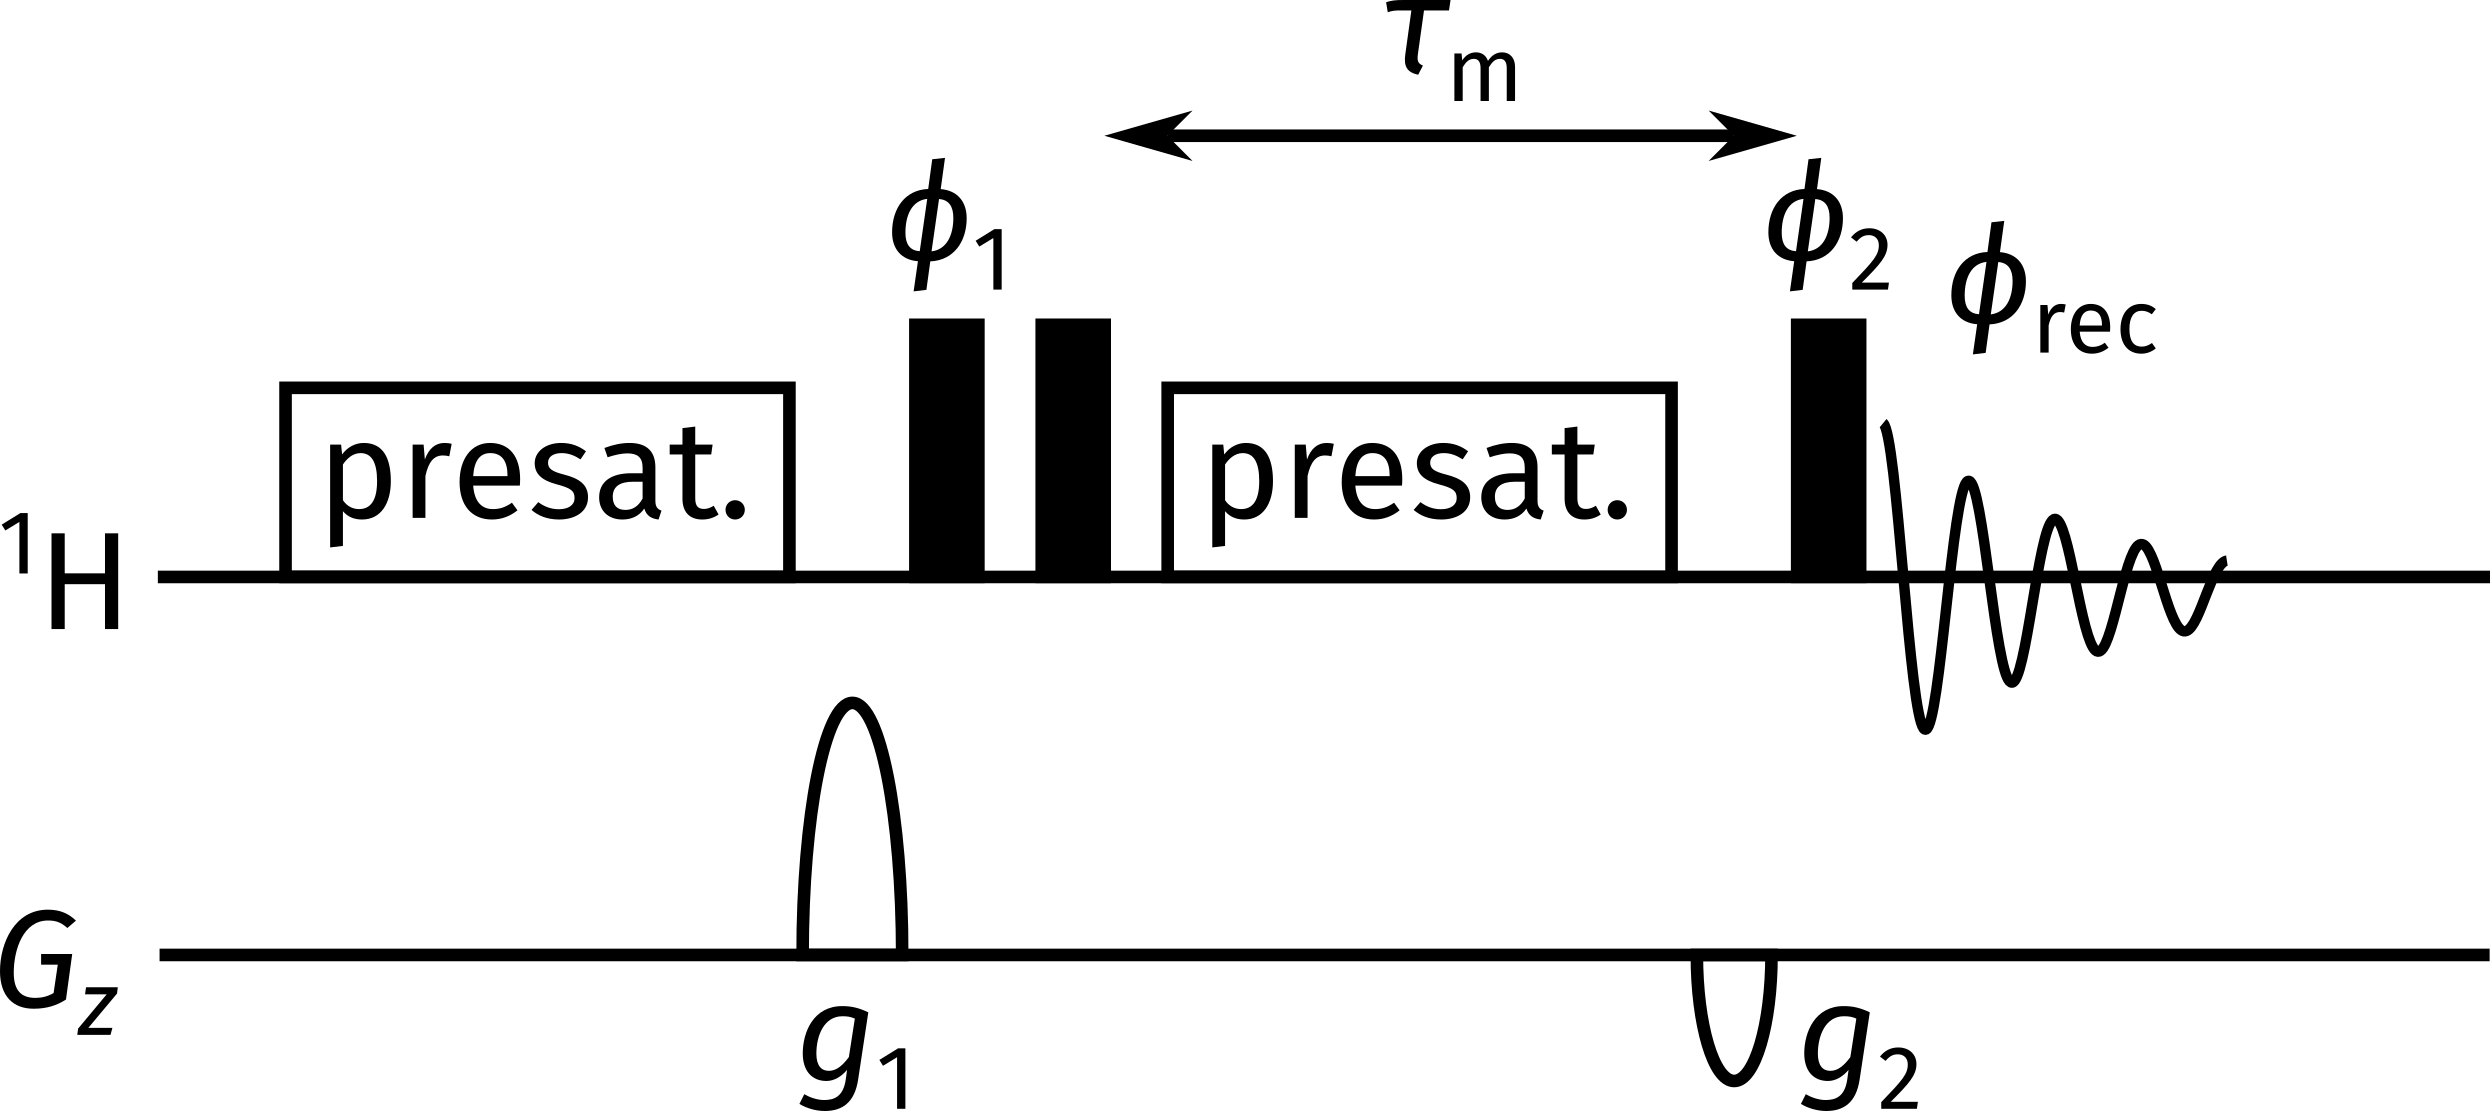
\includegraphics[draft=false]{pp/noesygppr1d.png}%
    \caption[1D NOESY pulse sequence for water suppression]{
        1D NOESY pulse sequence used for water suppression.
        Presaturation of the water resonance is applied during the recovery delay as well as the NOE mixing time.
        Phase cycling is performed with $\phi_1 = (x, -x)$, $\phi_2 = (x, x, -x, -x, y, y, -y, -y)$, and $\phi_\text{rec} = (x, -x, -x, x, y, -y, -y, y)$.
        Gradient amplitudes are $(g_1, g_2) = (50\%, -10\%)$.
        Boxes labelled with `presat.' indicates periods of weak presaturation.
    }
    \label{fig:poise_solvsupp_pulseq}
\end{figure}


\subsubsection{Optimisation setup}

In a similar style to the PSYCHE optimisations (\cref{subsec:poise__psyche}), a series of optimisations with increasing numbers of parameters were run.
However, in this case, the cost function is far easier to construct and far less noisy: we can simply integrate the water peak, which was defined to be the region of the spectrum between 4.65 and \SI{4.75}{\ppm}, and use that (or its absolute value) as the cost function.
In practice, because the phase of the water peak can vary rather unpredictably, I preferred to reuse the sum-of-squares cost function $f_\text{sos}$ (\cref{eq:sos_cost_function}).
Squaring each point of the spectrum not only accounts for the possible sign changes, but also more strongly penalises intense absorption-mode water peaks which are more likely to obscure nearby peaks.

One drawback of the water suppression optimisation is that the phase cycle of the 1D NOESY is integral to its performance: thus, several scans must be used for a reliable cost function to be obtained, making for relatively long optimisations.
In this case, I used \texttt{DS=2} and \texttt{NS=4}.

A sample of rodent urine in \ch{D2O} was used, kindly provided by Abi Yates and Fay Probert (both University of Oxford).



\subsubsection{Optimisation results}

As before, I first provide a `summary' table comparing the optimisations with different numbers of parameters (\cref{tbl:poise_solvsupp_summary}).
From this, we see a similar story to before, in that optimising more parameters takes more time but leads to larger decreases in the cost function.
Individual details of each set of optimisations are given in \cref{tbl:poise_solvsupp1p,tbl:poise_solvsupp2p,tbl:poise_solvsupp3p,tbl:poise_solvsupp4p}.

The corresponding spectra post-optimisation are shown in \cref{fig:poise_solvsupp_spec}.
Clearly, the optimisations succeed in reducing the size of the water peak, especially the four-parameter optimisation.
However, perhaps equally importantly, the doublet at \SI{4.56}{\ppm} is unaffected by the optimisation.
Since the cost function does not actually check for the retention of peaks outside the target window, it is in principle possible that the optimisation will converge to parameters which achieve excellent water suppression but also cause nearby peaks to be lost.
This possibility is averted here by setting a conservative upper bound of \SI{55}{\Hz} on the presaturation power $k$: this avoids inadvertently saturating nearby resonances.

In fact, it may be justifiable in this case to run a long, four-parameter optimisation (which takes around 30 minutes), especially if many samples are to be run using the same optimised water suppression parameters.
However, for more routine usage, it is probably preferable to limit the number of parameters being optimised to two.


\begin{table}
    \centering
    \begin{tabular}{cccccccc}
        \toprule
         & \multicolumn{3}{c}{Aggregated results from all runs} & \multicolumn{4}{c}{Parameters from best optimum} \\
        Description & $f_\mathrm{sos} / 10^{18}$ & FEs & Time (\si{\s}) & $\nu_\text{tx}$ (\si{\Hz}) & $k$ (\si{\Hz}) & $\taum$ (\si{\s}) & $\taur$ (\si{\s}) \\
        \hline
        Initial point & 14.7         & --     & --         & (1880.61) & (50.0) & (0.100) & (2.00) \\
        1 parameter   & 1.85--2.49   & 6--12  & 259--520   & 1880.41   & (50.0) & (0.100) & (2.00) \\
        2 parameters  & 1.21--9.68   & 9--21  & 390--911   & 1880.20   & 51.94  & (0.100) & (2.00) \\
        3 parameters  & 1.24--4.20   & 19--26 & 825--1128  & 1879.90   & 47.79  & 0.118   & (2.00) \\
        4 parameters  & 0.165--1.65  & 25--53 & 1143--2314 & 1881.10   & 53.28  & 0.150   & 3.00 \\
        \hline
    \end{tabular}
    \caption[Overview of all water suppression optimisations]{
        Summary of optimisations on 1D NOESY / presaturation pulse sequence for water suppression.
        Parameters in parentheses were not optimised and were simply carried over from the initial point.
        A detailed breakdown of the results by algorithm, as well as the POISE routines used, are described in \cref{tbl:poise_solvsupp1p,tbl:poise_solvsupp2p,tbl:poise_solvsupp3p,tbl:poise_solvsupp4p}.
        \datacode{4P-210620}
    }
    \label{tbl:poise_solvsupp_summary}
\end{table}

\begin{figure}[htb]
    \centering
    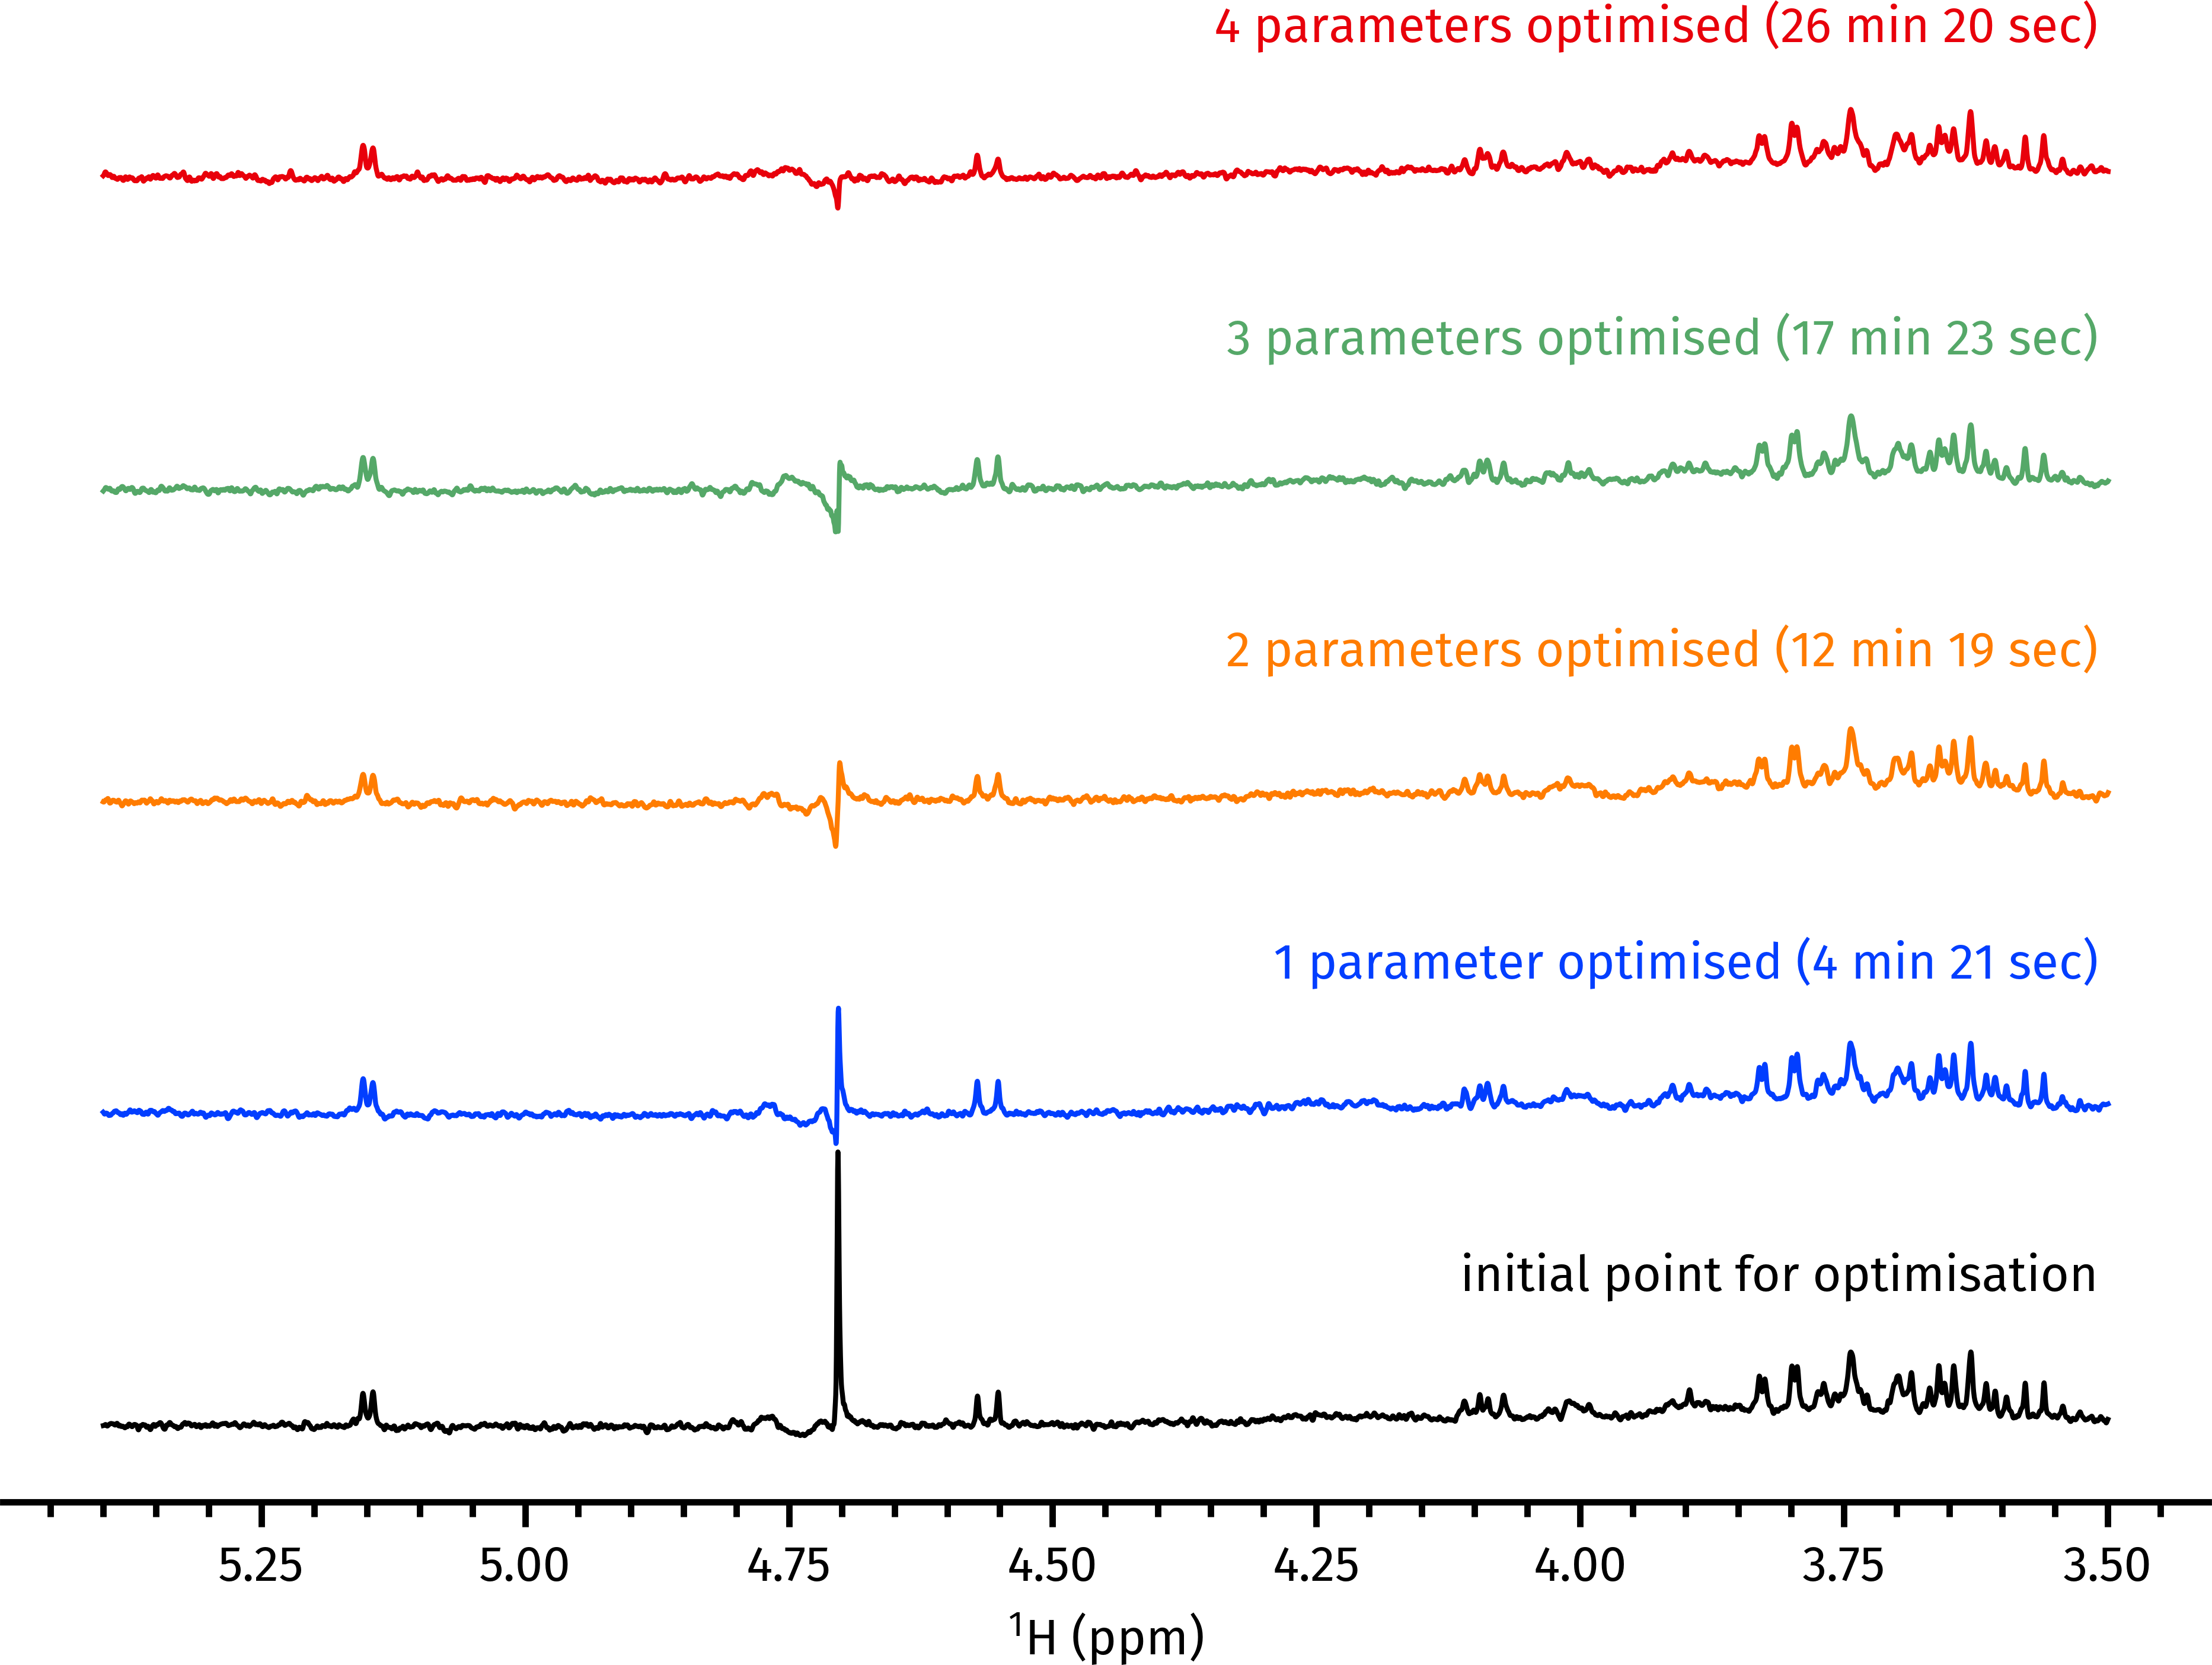
\includegraphics[draft=false]{poise/solvsupp_spec.png}
    \caption[1D NOESY spectra of rodent urine sample before and after optimisation]{
        Insets of 1D NOESY spectra acquired using optimised parameters from each set of optimisations in \cref{tbl:poise_psyche_summary}; the time required to obtain the optimised parameters is also indicated for each spectrum.
        The sample used was rodent urine in \ch{D2O}.
        Note that, for the 3- and 4-parameter optimisations, the best optimum from the 15 runs (i.e.\ the optima listed in \cref{tbl:poise_solvsupp_summary}) was used to acquire the spectra shown here.
        However, this was not the case for the 2-parameter optimisation: I (inexplicably) used a different optimum.
        This was probably an oversight on my part.
        Nevertheless, it does not affect any of the conclusions drawn here.
        \datacode{4P-210620}
    } \label{fig:poise_solvsupp_spec}
\end{figure}

\begin{table}
    \hbadness=10000
    \centering
    \begin{tabular}{ccccc}
        \toprule
        Entry & Algorithm & Optimum found (\si{\Hz}) & FEs    & Time taken (\si{\s}) \\
        \midrule
        1     & NM        & 1880.24--1880.49         & 10--12 & 436--519             \\
        2     & MDS       & 1880.24--1880.36         & 12     & 518--520             \\
        3     & BOBYQA    & 1880.34--1880.47         & 6--7   & 259--303             \\
        \bottomrule
    \end{tabular}
    \caption{
        Water suppression 1-parameter (transmitter offset) optimisations.
        The POISE routine used was: \mintinline[breaklines]{json}{{"name": "solvsupp1", "pars": ["o1"], "lb": [1870.61], "ub": [1890.61], "init": [1880.61], "tol": [0.2], "cf": "zerorealint_squared", "au": "poise_1d_noapk"}}.
        \datacode{4P-210620}
    }
    \label{tbl:poise_solvsupp1p}
\end{table}

\begin{table}
    \hbadness=10000
    \centering
    \begin{tabular}{ccccccc}
        \toprule
              &           & \multicolumn{3}{c}{Best optimum found} & \multicolumn{2}{c}{Aggregated results} \\
                            \cmidrule(lr){3-5}                       \cmidrule(lr){6-7}
        Entry & Algorithm & $\nu_\text{tx}$ (\si{\Hz}) & $k$ (\si{\Hz}) & $f_\text{sos} / 10^{18}$ & FEs    & Time (\si{\s}) \\
        \midrule
        1     & NM        & 1880.20                    & 51.94          & 1.209                    & 17--21 & 737--911       \\
        2     & MDS       & 1880.85                    & 50.81          & 2.600                    & 15     & 649--652       \\
        3     & BOBYQA    & 1881.12                    & 50.03          & 2.887                    & 9--14  & 390--608       \\
        \bottomrule
    \end{tabular}
    \caption{
        Water suppression 2-parameter (transmitter offset and presaturation power) optimisations.
        The POISE routine used was: \mintinline[breaklines]{json}{{"name": "solvsupp2", "pars": ["o1", "cnst20"], "lb": [1870.61, 10.0], "ub": [1890.61, 55.0], "init": [1880.61, 50.0], "tol": [0.2, 2.5], "cf": "zerorealint_squared", "au": "poise_1d_noapk"}}.
        \datacode{4P-210620}
    }
    \label{tbl:poise_solvsupp2p}
\end{table}

\begin{table}
    \hbadness=10000
    \centering
    \begin{tabular}{cccccccc}
        \toprule
              &           & \multicolumn{4}{c}{Best optimum found} & \multicolumn{2}{c}{Aggregated results} \\
                            \cmidrule(lr){3-6}                       \cmidrule(lr){7-8}
        Entry & Algorithm & $\nu_\text{tx}$ (\si{\Hz}) & $k$ (\si{\Hz}) & $\taum$ (\si{\ms}) & $f_\text{sos} / 10^{18}$ & FEs    & Time (\si{\s}) \\
        \midrule
        1     & NM        & 1879.90                    & 47.79          & 117.7              & 1.238                    & 23--26 & 1002--1128     \\
        2     & MDS       & 1882.79                    & 52.95          & 49.91              & 1.843                    & 24--25 & 1034--1080     \\
        3     & BOBYQA    & 1881.85                    & 52.14          & 134.7              & 1.738                    & 19--26 & 825--1133      \\
        \bottomrule
    \end{tabular}
    \caption{
        Water suppression 3-parameter (transmitter offset, presaturation power, and mixing time) optimisations.
        The POISE routine used was: \mintinline[breaklines]{json}{{"name": "solvsupp3", "pars": ["o1", "cnst20", "d8"], "lb": [1870.61, 10.0, 0.010], "ub": [1890.61, 55.0, 0.150], "init": [1880.61, 50.0, 0.100], "tol": [0.2, 2.5, 0.010], "cf": "zerorealint_squared", "au": "poise_1d_noapk"}}.
        \datacode{4P-210620}
    }
    \label{tbl:poise_solvsupp3p}
\end{table}

\begin{table}
    \hbadness=10000
    \centering
    \begin{tabular}{ccccccccc}
        \toprule
              &           & \multicolumn{5}{c}{Best optimum found} & \multicolumn{2}{c}{Aggregated results} \\
                            \cmidrule(lr){3-7}                       \cmidrule(lr){8-9}
        Entry & Algorithm & $\nu_\text{tx}$ (\si{\Hz}) & $k$ (\si{\Hz}) & $\taum$ (\si{\ms}) & $\taur$ (\si{\s}) & $f_\text{sos} / 10^{18}$ & FEs    & Time (\si{\s}) \\
        \midrule
        1     & NM        & 1880.72                    & 49.73          & 110.6              & 1.972             & 1.008                    & 29--40 & 1250--1726     \\
        2     & MDS       & 1882.65                    & 53.41          & 69.46              & 2.137             & 1.199                    & 34--53 & 1487--2314     \\
        3     & BOBYQA    & 1881.10                    & 53.28          & 150.0              & 3.000             & 0.1653                   & 25--40 & 1143--1843     \\
        \bottomrule
    \end{tabular}
    \caption{
        Water suppression 4-parameter (transmitter offset, presaturation power, mixing time, and presaturation duration) optimisations.
        The POISE routine used was: \mintinline[breaklines]{json}{{"name": "solvsupp4", "pars": ["o1", "cnst20", "d8", "d1"], "lb": [1870.61, 10.0, 0.010, 1.0], "ub": [1890.61, 55.0, 0.150, 3.0], "init": [1880.61, 50.0, 0.100, 2.0], "tol": [0.2, 2.5, 0.010, 0.1], "cf": "zerorealint_squared", "au": "poise_1d_noapk"}}.
        \datacode{4P-210620}
    }
    \label{tbl:poise_solvsupp4p}
\end{table}




\subsubsection{Optimisation on a sucrose sample}

The water suppression optimisations shown above were in fact developed and first evaluated on a sample of sucrose in 90\% \ch{H2O}/10\% \ch{D2O}.
This sample is less `interesting' in that there are no resonances close to the water peak, and I also did not perform replicates of each optimisation run (this data never made it into the POISE paper).
Nevertheless, I still believe it is still worth adding the results here, as they demonstrate that the optimisation procedure can be easily applied to different samples.
Furthermore, the suppression requirements are even more demanding here because there is simply more water present.

In this case, the one-parameter optimisation seemed to have no significant effect on the result: this is possibly because the initial value chosen for that single parameter (the transmitter offset) already happened to be an optimum.
However, the two- through four-parameter optimisations all yielded significant improvements in the water suppression (\cref{fig:poise_solvsupp_sucrose_spec}).

\begin{figure}[htb]
    \centering
    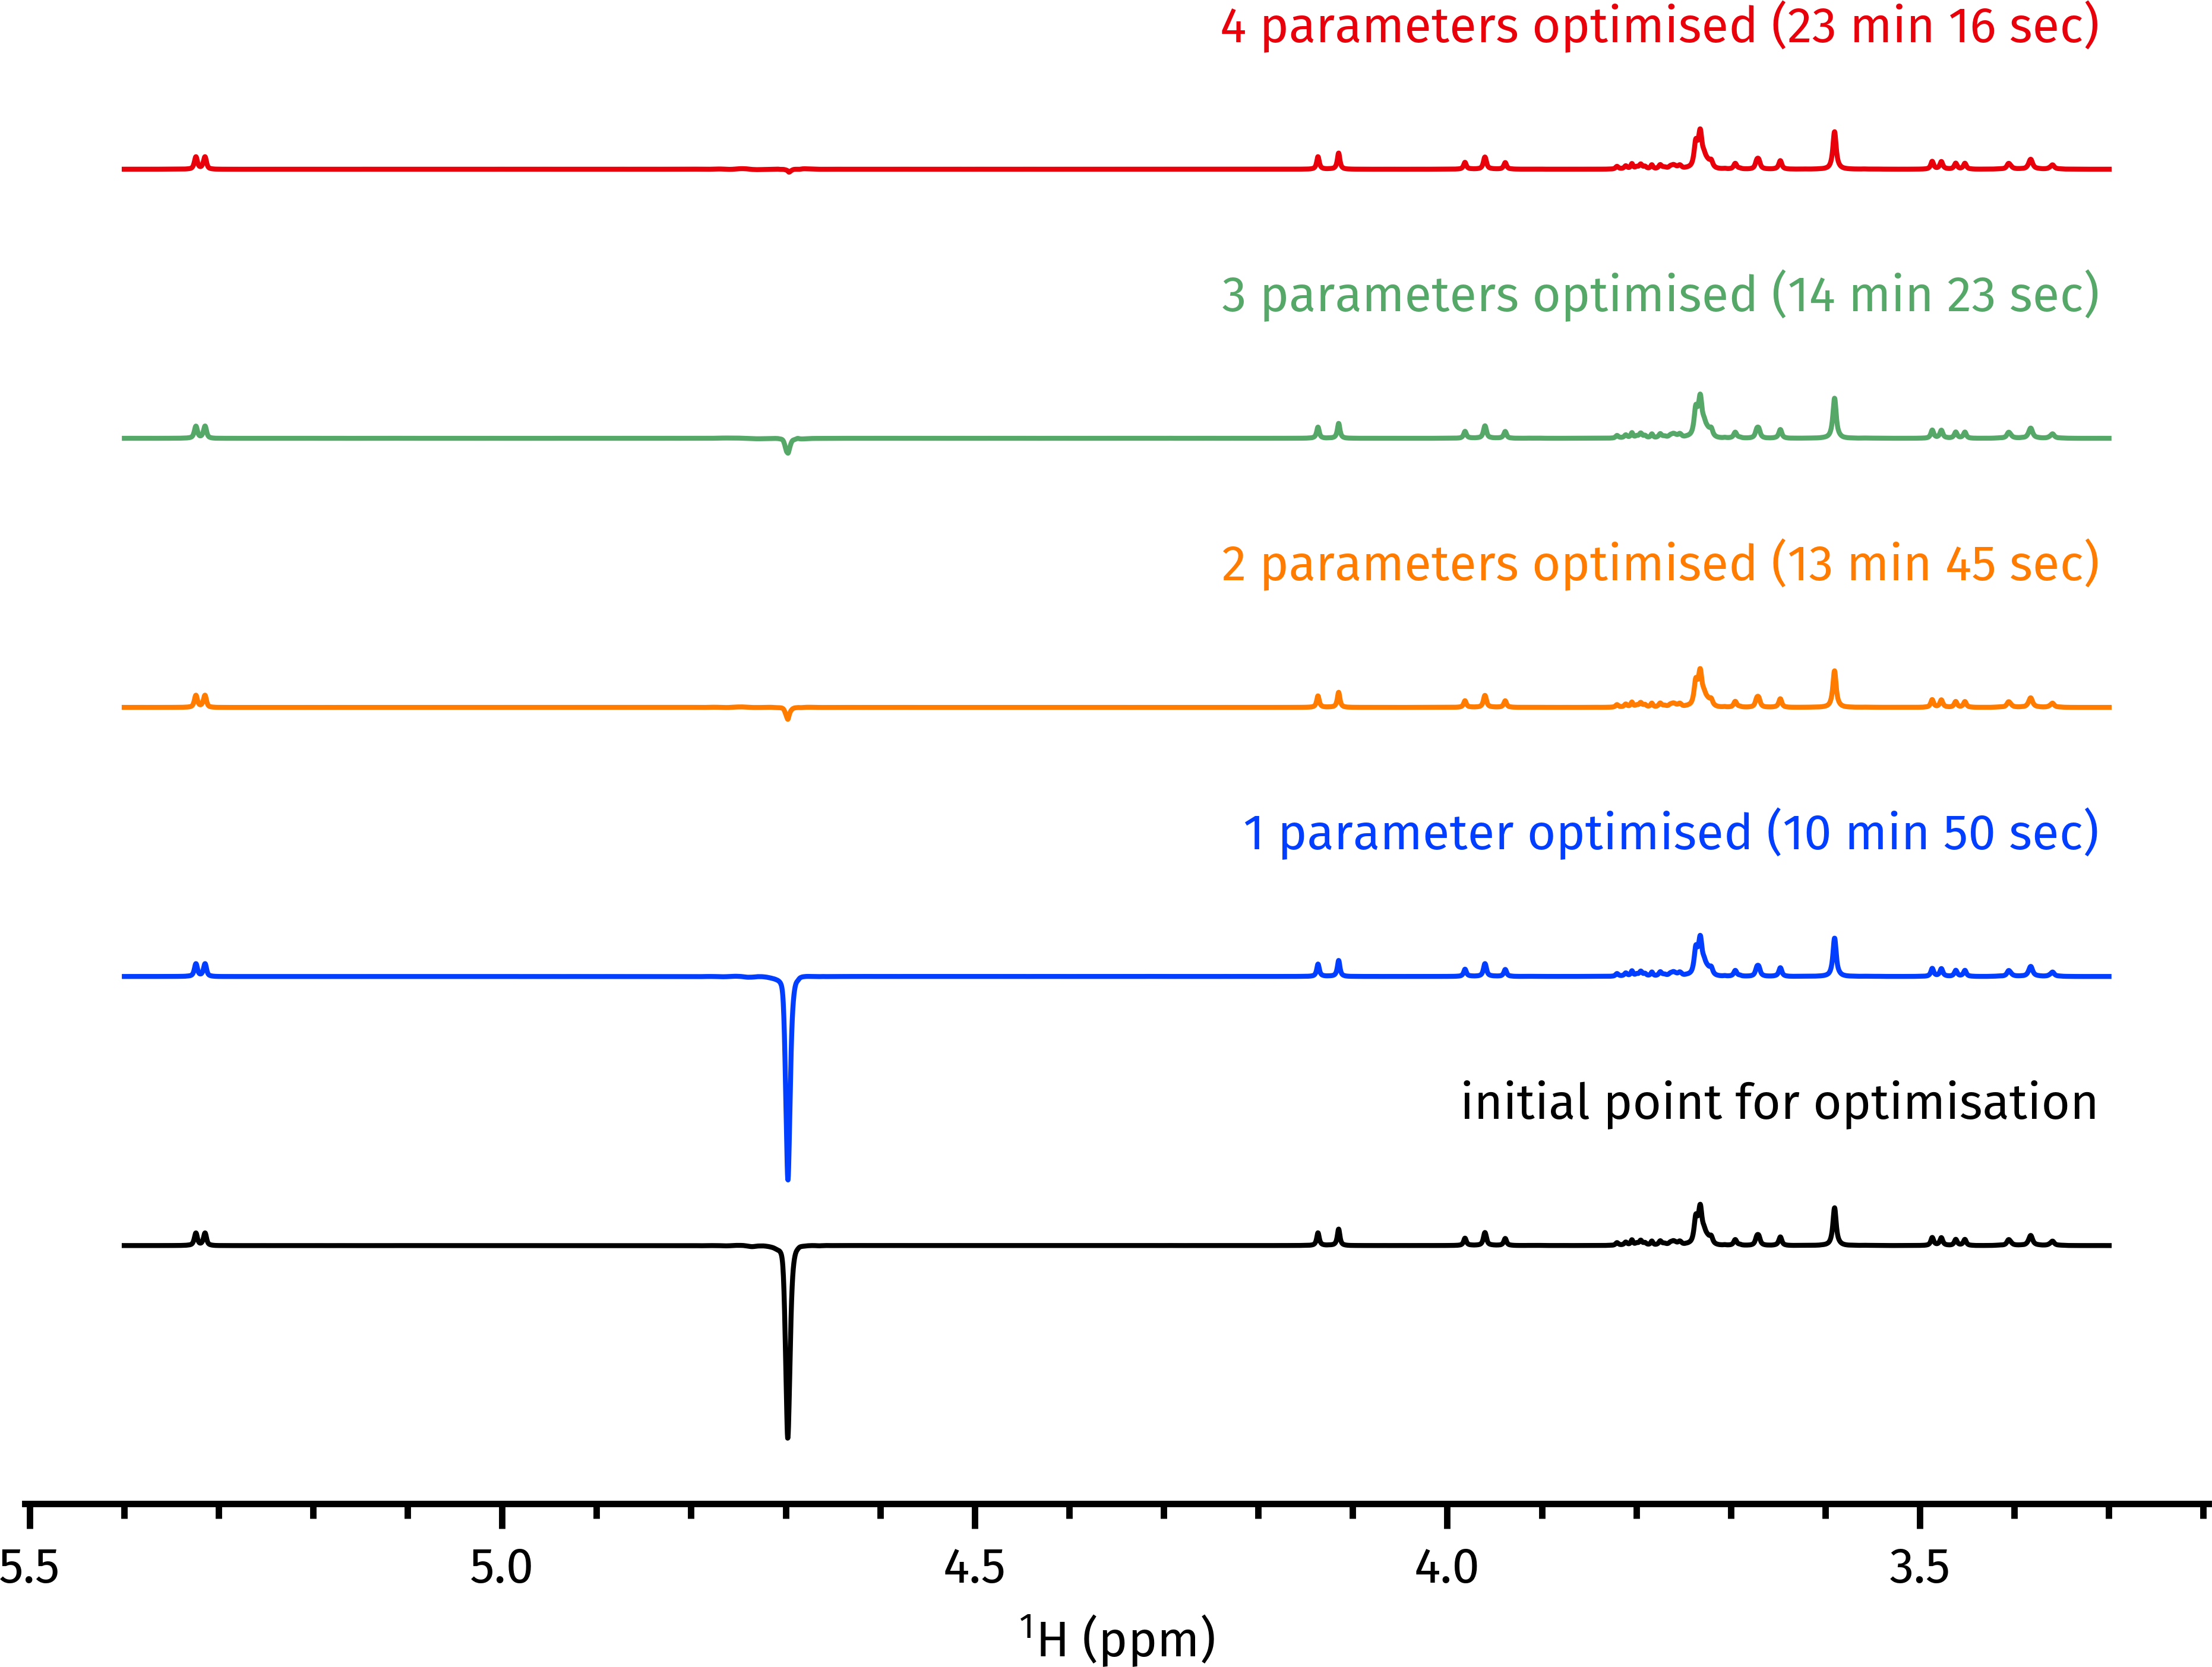
\includegraphics[draft=false]{poise/solvsupp_sucrose_spec.png}
    \caption[1D NOESY spectra of sucrose sample before and after optimisation]{
        Insets of 1D NOESY spectra acquired after optimisation of 1, 2, 3, or 4 parameters (the exact parameters being optimised are the same as in \cref{fig:poise_solvsupp_spec}).
        The sample used was sucrose in 90\% \ch{H2O}/10\% \ch{D2O}.
        The time required to obtain the optimised parameters is also indicated for each spectrum.
        \datacode{4S-210617}
    }
    \label{fig:poise_solvsupp_sucrose_spec}
\end{figure}
